% report_31_01_2018.tex
% Omkar H. Ramachandran
% omkar.ramachandran@colorado.edu
%
% Documentation for hemispheric dependence in the Fermi Pass 8 data
%

\chapter{Preparation and Analysis of Fermi Data}
%\begin{figure}
%	\centering
%	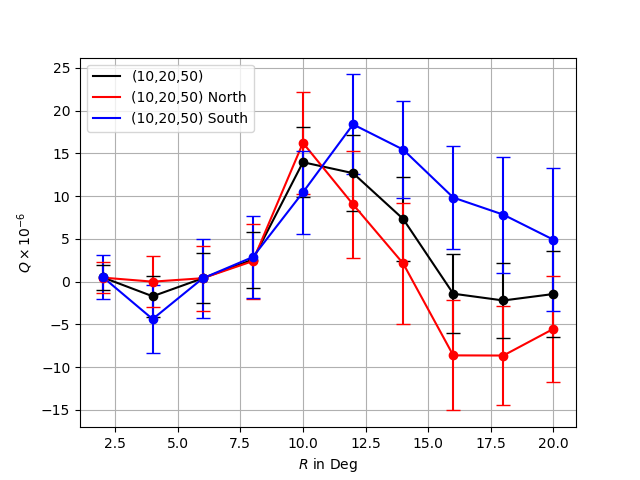
\includegraphics[scale=0.5]{Qhemisphere_wk_100_400_10_20_50_scrubbed.png}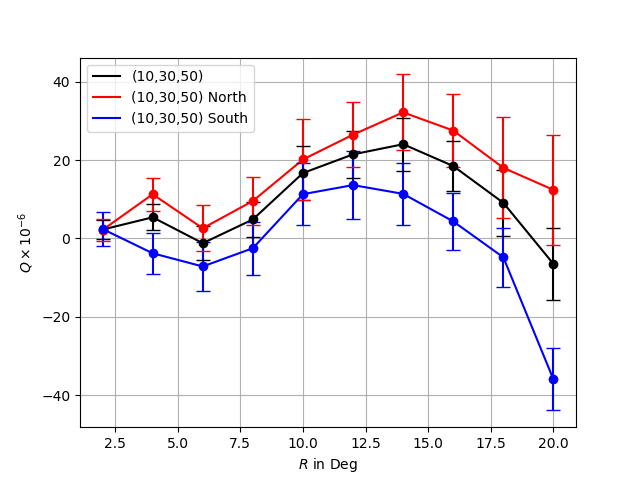
\includegraphics[scale=0.5]{Qhemisphere_wk_100_400_10_30_50_scrubbed.png}
%
%	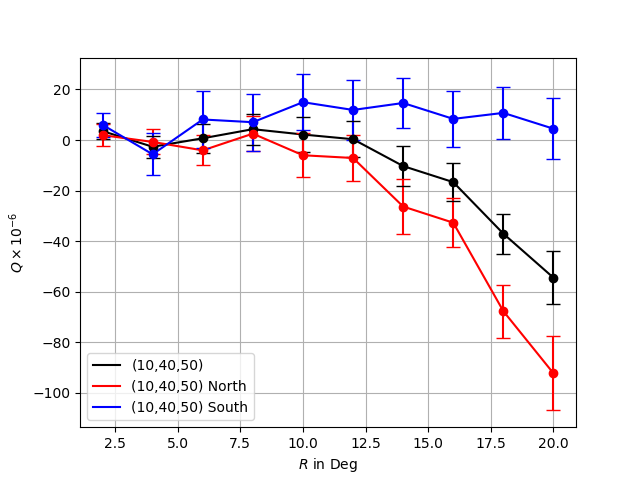
\includegraphics[scale=0.5]{Qhemisphere_wk_100_400_10_40_50_scrubbed.png}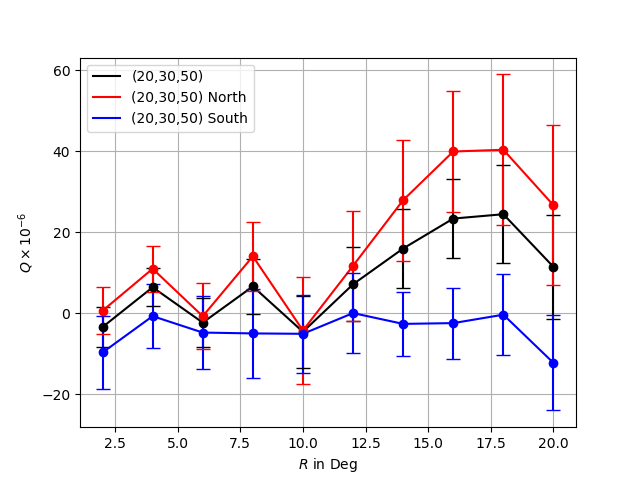
\includegraphics[scale=0.5]{Qhemisphere_wk_100_400_20_30_50_scrubbed.png}
%	
%	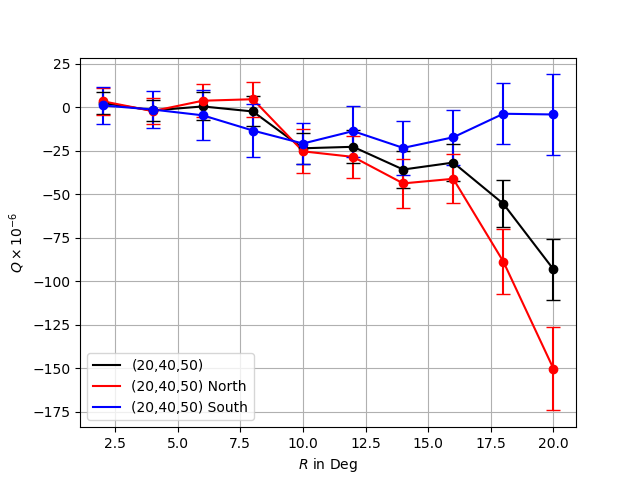
\includegraphics[scale=0.5]{Qhemisphere_wk_100_400_20_40_50_scrubbed.png}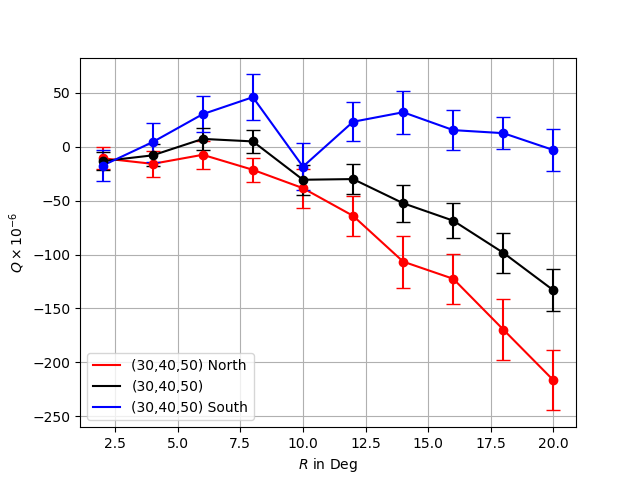
\includegraphics[scale=0.5]{Qhemisphere_wk_100_400_30_40_50_scrubbed.png}
%	\caption{(Clockwise from top) Plot of computed value of $Q$ as a function
%	of $R$ for (a) 10,20,50 (b) 10,30,50 (c) 20,30,50 (d) 30,40,50 (e) 20,40,50
%	and (f) 10,40,50}
%	\label{fig:hemisphere}
%\end{figure}

\section{Outline of Filtering method}
The predictions made in the Tashiro et al. (2014) -- and later in Chen et al.
(2015) -- assumed that the photons involved in computing $Q$ originited
purely from extragalactic sources. 
Going back to the mean free path of $\TeV$ photons defined in 
Tashiro \& Vachaspati (2013), we have the following:
$$ D_{\TeV} \propto 80\left(\frac{E_{\TeV}}{10 \TeV}\right)^{-1}\ \Mpc$$
\begin{equation}
	\implies D_{\TeV} \sim 80\left(\frac{E_{\gamma}}{88\ \GeV}\right)^{-1/2}\ \Mpc
\end{equation}
In essence, an upscattered photon with $E \sim 50\ \GeV$ likely originated
from a source that travelled an average of $80\ \Mpc$ before the scattering event.
As a result, we can already pin down a major source of noise in the high energy 
photons originating from the galactic disk.
Similarly, photons originating from scattering events in the upper atmosphere
also had to be filtered for.
In all, we scrubbed the raw data using the following constraints -- mostly
following the procedure used in Tashiro et al (2014) and later Chen et al (2015):
\begin{itemize}
\item For measuring $Q$, we used $404$ weeks of data from Pass 8 of the Fermi 
	LAT, specifically, from weeks 100 through 504.
\item To avoid contamination from the galactic disk, we constrained photons in
	the highest energy bin present to the region on the sky described by 
	$b > 70^{\circ}$. We later tightened the constraint to $b > 80^{\circ}$, 
	further increasing the likelihood that the photons used in the analysis.  
\item To avoid contamination from cosmic ray scattering in the upper
	atmosphere, photons arriving at Zenith angles greater than $100^{\circ}$ 
	were discarded.
\item Finally, the selected data with these characteristics was filtered so as
	to only use photons that were marked as 'CLEAN' or 'ULTRACLEAN'
	using the 'gtmktime' command in the sciencetools package. 
	Chen et al. (2015) tightened the constraint to only use 'ULTRACLEAN' photons,
	but our early analysis suggested that there was very little difference in the
	signal -- this was also observed by Chen et al. (2015) --, and thus we 
	allowed for both CLEAN and ULTRACLEAN to increase the overall observed 
	flux of high energy photons.
\item The spacecraft's rocking angle at the time of event detection was also 
	constrained to a maximum of $52^{\circ}$.
\end{itemize}

\section{Distribution of points}

\section{Computing $Q$ from filtered data}
As elaborated in Section (insert ref here), the pseudoscalar we wish to compute is
the following:
\begin{equation}
	Q(R,E_{1},E_{2},E_{3}) = \frac{1}{N_3}\sum_{k=1}^{N_{3}}\eta_1\times\eta_2
	.\eta_k(E_3)
\end{equation}
where $\eta_a = (1/N_a)\sum_{i\in D(\eta_k,R)} \eta_{i}(E_a)$, $a={1,2}$ and 
$D(\eta_k,R)$ implies that only photons in the $E_1$ and $E_2$ bin that lie
within a patch of radius $R$ around any given $E_3$ photon are to be used in
the computation.
Of course, the fastest way to do this computation -- discussed in further detail 
in Appendix (insert ref) -- is to perform all the summmation first for each of 
the three vectors and then do one triple product for the resulting sums.
This reduces the overall complexity of the routine from $O(N^{3})$ to $O(N)$.
For each $Q(R)$ computed, we computed standard errors as follows:
\begin{equation}
	\sigma_Q(R) = \frac{\sigma(Q(R,E_{3}))}{\sqrt{N_3}}
	\label{eq:standard_error}
\end{equation}
In essence, we define the error as simply the standard deviation of triple products
at a given radius for a given photon in $E_{3}$, normalized by the number of photons
in $E_{3}$ within the patch.
There is one major issue with this approach:
Computing the standard error as in equation (\ref{eq:standard_error}) assumes 
that $Q(R=R_{j})$ is independant of $Q(R \neq R_{j})$, which isn't true. 
Computing $Q(R=4^{\circ})$, for instance, will necesasrily contain every 
triple product in $Q(R < 4^{\circ})$.
Therefore, while we present plots with error-bars defined by $\sigma_Q(R)$,
we also manually compute the probability of the observed curve appearing in
the Monte-Carlo to further evidence any major statistical result.

\section{Results}
The goal of this section will be to present and compare the results of the
analysis routine described in the previous section.
For both $b(E_{3}) > 70^{\circ}$

\subsubsection{$E_1 = 10 \GeV$}
Looking at Figure \ref{fig:hemisphere}, we observe that for two of the three
energy combinations (10,20,50 and 10,30,50), the $Q$ vs $R$ curves for the 
northern and southern hemispheres track each other. 
For (10,40,50) however, we see sharp hemispheric dependence with a strong negative
trend for the curve in the northern hemisphere that isn't seen in the 
corresponding curve for the southern hemisphere.
As will be demonstrated in the remaining two sections, this dependence seems
to appear only in combinations that include the $40$ to $50$ $\GeV$ bin.

\subsubsection{$E_1 = 20 \GeV$}
Once again, we observe that only the bin combination with $40$ to $50$ $\GeV$
(Figure \ref{fig:hemisphere}(e)) shows sharp hemispheric dependence. 
For the remaining combinations, the overall value of $Q$ at $R=20$ is zero within
errorbars.

\subsubsection{$E_1 = 30 \GeV$}
When the lowest energy bin is set at $30 \GeV$, there is exactly one combination
that is possible: 30,40,50 (Figure \ref{fig:hemisphere}(d)).
Here, we observe that the curve is similar to 40,50 combination in the previous 
sections, with the northern curve being significantly more negative than the
southern curve.


\begin{figure}
	\centering
	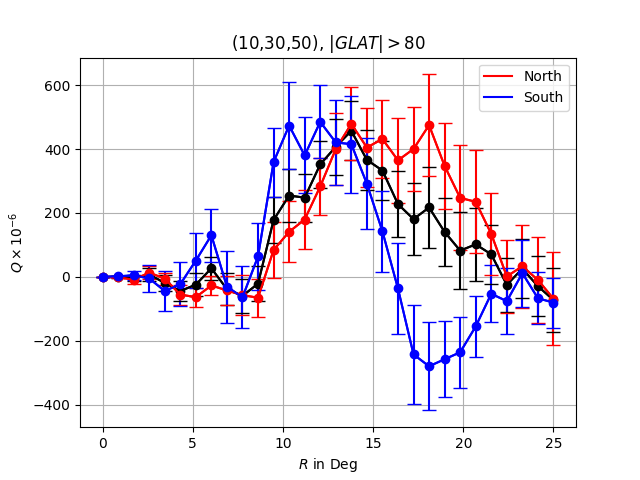
\includegraphics[scale=0.5]{10_30_50_full.png}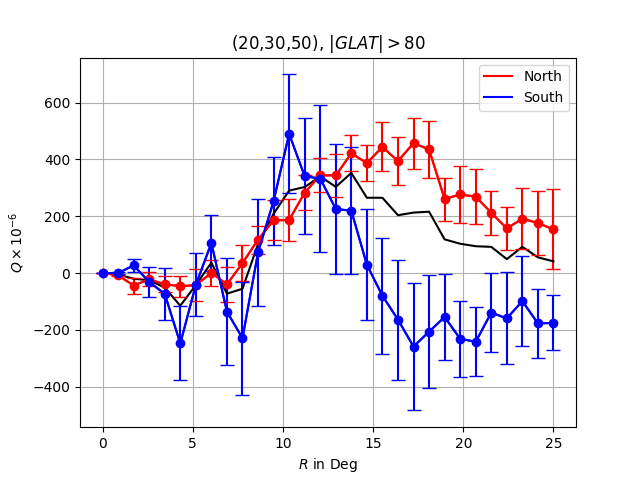
\includegraphics[scale=0.5]{20_30_50_full.png}
	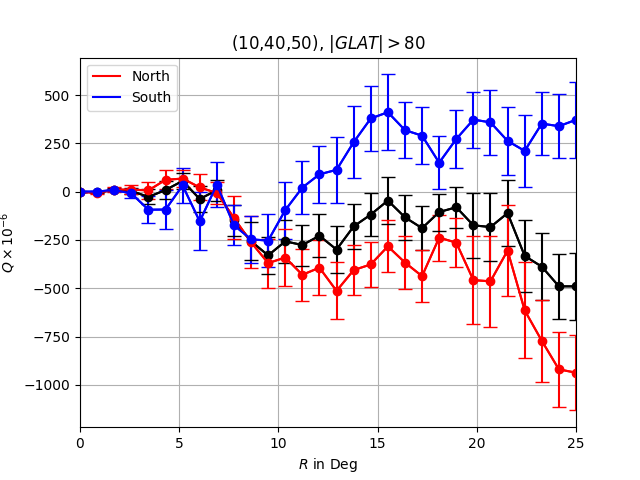
\includegraphics[scale=0.5]{10_40_50_full.png}
	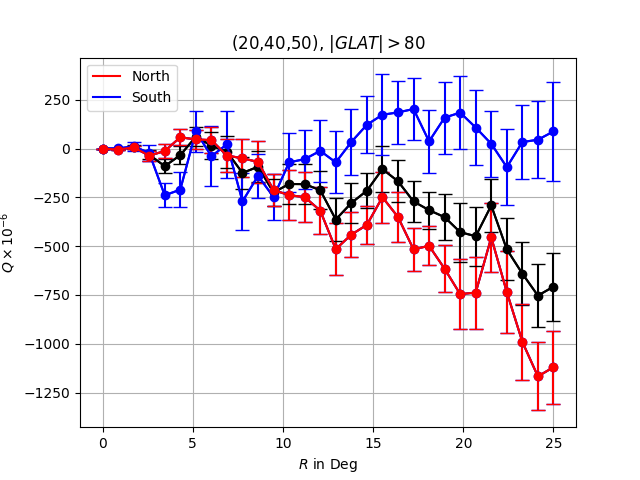
\includegraphics[scale=0.5]{20_40_50_full.png}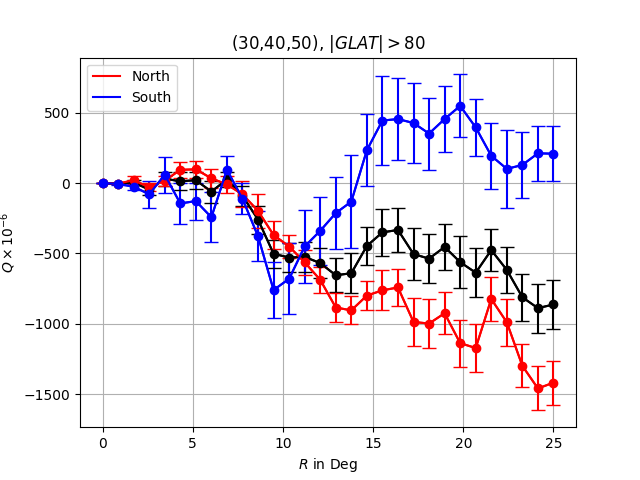
\includegraphics[scale=0.5]{30_40_50_full.png}

	\caption{Plots of $Q$ vs the patch radius $R$ around each $E_3$
	point for (top) $E_2 = 30\ \GeV$ and (middle and bottom) 
	$E_2=40\ \GeV$}
	\label{fig:hemisphere_lg80}
\end{figure}



\begin{figure}
	\centering
	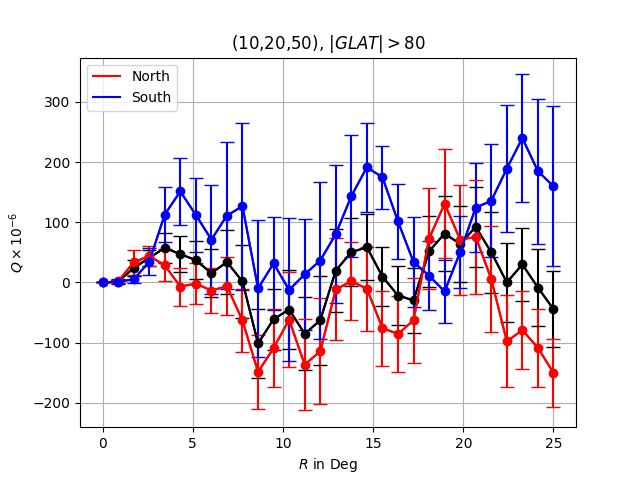
\includegraphics[scale=0.5]{10_20_50_full.png}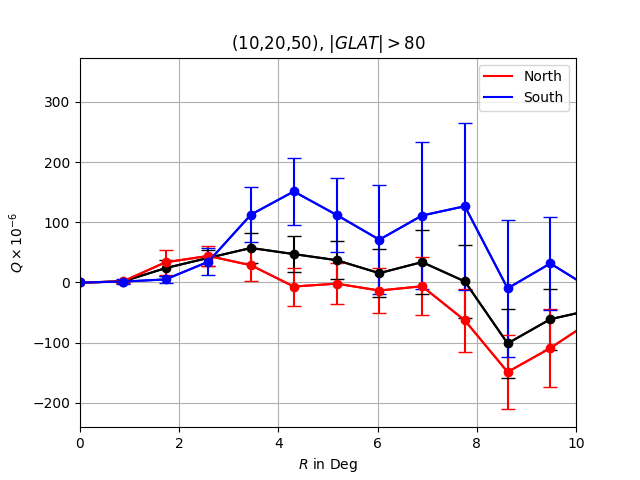
\includegraphics[scale=0.5]{10_20_50_upto_10.png}
	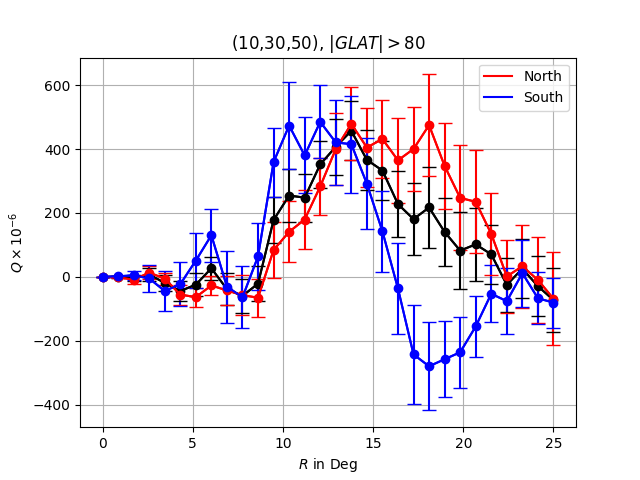
\includegraphics[scale=0.5]{10_30_50_full.png}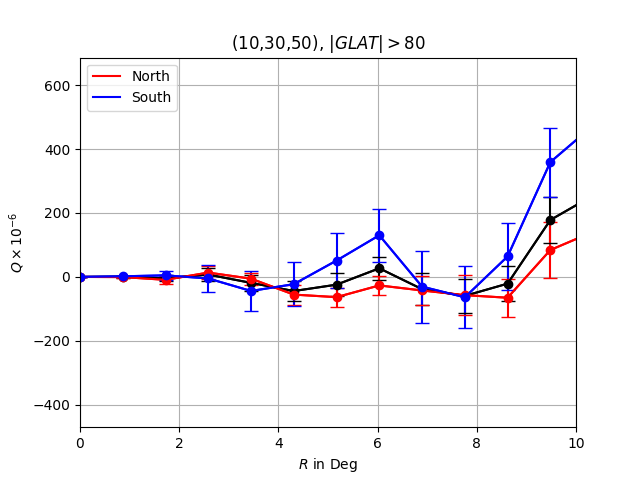
\includegraphics[scale=0.5]{10_30_50_upto_10.png}
	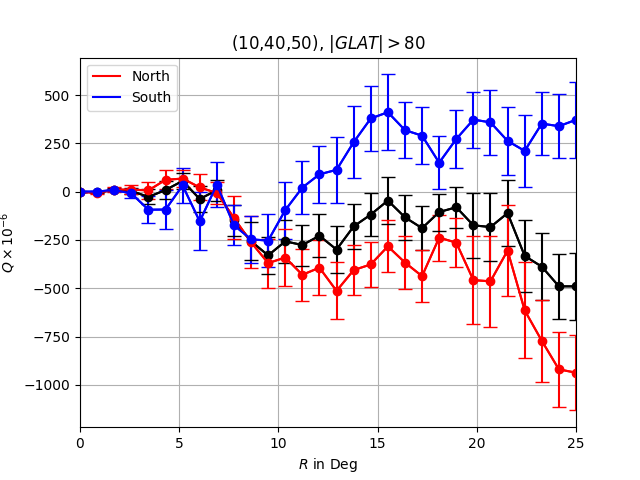
\includegraphics[scale=0.5]{10_40_50_full.png}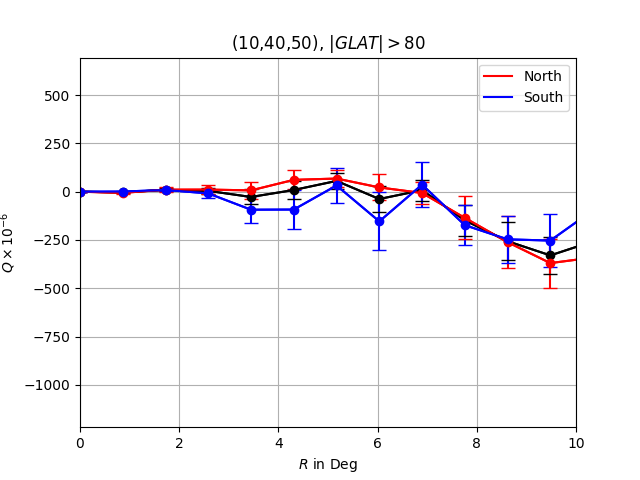
\includegraphics[scale=0.5]{10_40_50_upto_10.png}

	\caption{(Top to bottom) Plots of $Q$ vs the patch radius $R$ around each $E_3$
	point for (left) $R\in[0^{\circ},25^{\circ}]$ and (right) 
	$R\in[0^{\circ},10^{\circ}]$, $E_{1} = 10\ \GeV$ and $l>80^{\circ}$}
	\label{fig:hemisphere_lg80}
\end{figure}



\subsection{$l_{E_3} > 80^{\circ}$}
When we restrict our patches to points in the $E_{3}$ energy bin that are higher
than $|l| > 80^{\circ}$.
In this scenario, we see that there are two distinct regimes for all but one of
the energy bin combinations (10,20,50) Figure \ref{fig:hemisphere_lg80}.1.
Specifically, we observe that when we consider $R\leq10^{\circ}$ -- thus 
purely constraining ourselves to latitudes where the galactic disk is
expected to have minimal impact --, there is no hemispheric dependance.
As in section 2.1, we observe that the intermediate bin is a very good
predictor of the $Q$ vs $R$ trend (Figure \ref{hemisphere_lg80}).
We also find that $Q$ is weakly positive or zero under these circumstances
for $E_{2}\in{20,30}\ \GeV$ and is strongly negative only for 
$E_2=40\ \GeV$.
This result further evidences the possibility that the hemispheric dependence
seen at high $R$ for the $l_{E_3}\geq70^{\circ}$ case is simply a case
of interference from the galactic disk, but we would need a full model of 
the galactic disk added into the Monte-Carlo simulation to confirm this
possibility.

\section{Discussion}
In each of the three cases discussed in the previous section, we observe that
the strong negative trend for $Q$ as well as the sharp hemispheric dependence
seems to appear only in the ($E_1$,40,50) bin. 
This might point to contamination in the $40$ to $50$ $\GeV$ bin that hasn't 
been accounted for in this setup, or it might point to some interesting 
physics.
Having said this, in each of the cases presented above, we find that the 
deviation between the measured overall value and the northern and southern
curve is at least $\sigma$ - with the exception of Figure 2(a).
Interestingly, the overall value of $Q$ is sharply negative only when we 
include the $40-50\ \GeV$ bin.
In all other cases, $Q$ is either weakly positive, or zero within error bounds.

